% The Fano plane P^2(F_2): 7 points, 7 lines (6 segments and the circle), 3 points on each line.
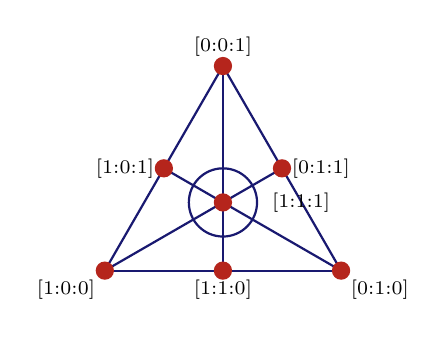
\begin{tikzpicture}[scale=1.5]
\draw[MidnightBlue,thick] (0.0000,0.0000) -- (2.0000,0.0000);
\draw[MidnightBlue,thick] (2.0000,0.0000) -- (1.0000,1.7321);
\draw[MidnightBlue,thick] (1.0000,1.7321) -- (0.0000,0.0000);
\draw[MidnightBlue,thick] (0.0000,0.0000) -- (1.5000,0.8660);
\draw[MidnightBlue,thick] (2.0000,0.0000) -- (0.5000,0.8660);
\draw[MidnightBlue,thick] (1.0000,1.7321) -- (1.0000,0.0000);
\draw[MidnightBlue,thick] (1.0000,0.5774) circle (0.2887);
\fill[BrickRed] (0.0000,0.0000) circle (2.2pt) node[below left,font=\scriptsize,black] {$[1{:}0{:}0]$};
\fill[BrickRed] (2.0000,0.0000) circle (2.2pt) node[below right,font=\scriptsize,black] {$[0{:}1{:}0]$};
\fill[BrickRed] (1.0000,1.7321) circle (2.2pt) node[above,font=\scriptsize,black] {$[0{:}0{:}1]$};
\fill[BrickRed] (1.0000,0.0000) circle (2.2pt) node[below,font=\scriptsize,black] {$[1{:}1{:}0]$};
\fill[BrickRed] (1.5000,0.8660) circle (2.2pt) node[right,font=\scriptsize,black] {$[0{:}1{:}1]$};
\fill[BrickRed] (0.5000,0.8660) circle (2.2pt) node[left,font=\scriptsize,black] {$[1{:}0{:}1]$};
\fill[BrickRed] (1.0000,0.5774) circle (2.2pt) node[right=0.5cm,font=\scriptsize,black] {$[1{:}1{:}1]$};
\end{tikzpicture}
